% tikzpic.tex
\documentclass[crop,tikz]{standalone}% 'crop' is the default for v1.0, before it was 'preview'
%\documentclass[tikz]{article}% 'crop' is the default for v1.0, before it was 'preview'
%\usepackage{tikz}
\usepackage{amsfonts}
\usepackage{amsmath}
%\usetikzlibrary{...}% tikz package already loaded by 'tikz' option

\usetikzlibrary{shapes}
\usetikzlibrary{arrows}
\usetikzlibrary{positioning}
\begin{document}
\newcommand{\word}{w}
\newcommand{\vocab}{\mathcal{V}}
\newcommand{\context}{\textsc{Context}}
\newcommand{\features}{\textsc{Features}}
\newcommand{\funcdef}[3]{#1 : #2 \rightarrow #3}
\newcommand{\rsubspace}[1]{\mathbb{R}^{#1}}
\newcommand{\elmo}{\textsc{Elmo} }
\newcommand{\wordImportance}{z}
\newcommand{\aggWordImportance}{\omega}
\newcommand{\sent}{s}

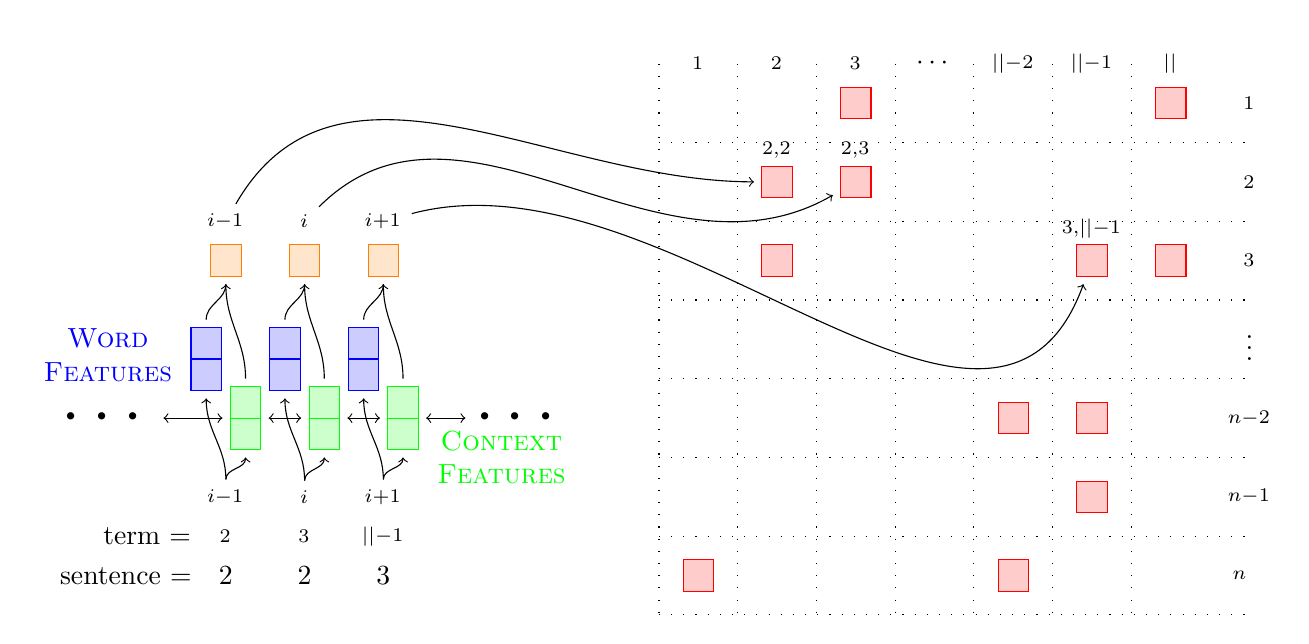
\begin{tikzpicture}[
  hid/.style 2 args={
    rectangle split,
    draw=#2,
    rectangle split parts=#1,
    fill=#2!20,
    outer sep=1mm},
  mlp/.style 2 args={
    rectangle split,
    rectangle split horizontal,
    draw=#2,
    rectangle split parts=#1,
    fill=#2!20,
    outer sep=1mm}
]



  \foreach \step in {1,...,7} {
     \draw [loosely dotted,black] (10.5, 10.5 - \step) to (18, 10.5 - \step);
     \draw [loosely dotted,black] (9.5 + \step, 10.5) to (9.5 + \step, 3.5);

  }

  \foreach \idx [count=\step] in {\vocab_2, \vocab_3, \vocab_{|\vocab|-1}} {
    \node (wv\step) at (\step + 5-1, 4.5) {$\idx$};
  }
  \foreach \idx [count=\step] in {2,2,3} {
    \node (sidx\step) at (\step + 5-1, 4) {$\idx$};
  }
    \node at (5-1,4.5) {term $=$} ;
    \node at (4.73-1,4) {sentence $=$} ;

  \foreach \idx [count=\step] in {i-1, i, i+1} {
    \node[hid={2}{blue}]      (ftr\step) at (\step + 5 - .25-1, 6.75) {}; 
    \node[hid={2}{green}]    (ctx\step) at (\step + 5 + .25-1, 6.00) {}; 
    \node[hid={1}{orange}] (score\step) at (\step + 5 + .00-1, 8.00) {}; 
    \node (w\step) at (\step + 5-1, 5.0) {$\word_{\idx}$};
    \node (z\step) at (\step + 5-1, 8.5) {$\wordImportance_{\idx}$};
     \draw [->,black] (w\step.north) to [out=90,in=-90] (ctx\step.south);
     \draw [->,black] (w\step.north) to [out=90,in=-90] (ftr\step.south);
     \draw [->,black] (ctx\step.north) to [out=90,in=-90] (score\step.south);
     \draw [-,black] (ftr\step.north) to [out=90,in=-90] (score\step.south);
     
  }
  
  \node (wpre) at (4.5-1, 6) {\Huge $\cdots$};
  \node (wpost) at (9.5 + .25-1, 6) {\Huge $\cdots$};
  \node[blue,align=center,text width=1.8cm] (ftrlbl) at (4.5-1, 6.8) 
    {\textsc{Word Features}};
  \node[green,align=center,text width=1.8cm] (ctxlbl) at (9.5-1, 5.5) 
    {\textsc{Context Features}};

  \foreach \next [count=\last] in {2, 3} {
    \draw [<->,black] (ctx\last) to (ctx\next); 
  }
  \draw [<->,black] (wpre.east) to (ctx1); 
  \draw [<->,black] (wpost.west) to (ctx3); 

  
%  \node (v1) at (18, 10) {$\vocab_1$};
%  \node (v2) at (18, 9) {$\vocab_2$};
%  \node (v3) at (18, 8) {$\vocab_3$};
%  \node (v4) at (18, 7) {$\vdots$};
%  \node (v5) at (18, 6.0) {$\vocab_{|\vocab|-2}$};
%  \node (v6) at (18, 5) {$\vocab_{|\vocab| - 1}$};
%  \node (v7) at (18, 4.0) {$\vocab_{|\vocab|}$};

  \node (v1) at (18, 10) {$\sent_1$};
  \node (v2) at (18, 9) {$\sent_2$};
  \node (v3) at (18, 8) {$\sent_3$};
  \node (v4) at (18, 7) {$\vdots$};
  \node (v5) at (18, 6.0) {$\sent_{n-2}$};
  \node (v6) at (18, 5) {$\sent_{n - 1}$};
  \node (v7) at (18, 4.0) {$\sent_{n~~}$};
 



  \node (s1) at (11.0, 10.5) {$\vocab_1$};
  \node (s2) at (12, 10.5) {$\vocab_2$};
  \node (s3) at (13, 10.5) {$\vocab_3$};
  \node (s4) at (14, 10.5) {$\cdots$};
  \node (s5) at (15, 10.5) {$\vocab_{|\vocab|-2}$};
  \node (s6) at (16, 10.5) {$\vocab_{|\vocab|-1}$};
  \node (s7) at (17, 10.5) {$\vocab_{|\vocab|}$};
  \node[hid={1}{red}] (wi1) at (12, 9) {};
  \node at (12,9.4) {$\aggWordImportance_{2,2}$};
  \node at (13,9.4) {$\aggWordImportance_{2,3}$};
  \node at (16,8.4) {$\aggWordImportance_{3, |\vocab|-1}$};
  \node[hid={1}{red}] (wi2) at (12, 8) {};
  \node[hid={1}{red}] (wi3) at (16, 8) {};
  \node[hid={1}{red}] (wi4) at (13, 10) {};
  \node[hid={1}{red}] (wi5) at (13, 9) {};
  \node[hid={1}{red}] (wi6) at (15, 6) {};
  \node[hid={1}{red}] (wi6) at (16, 6) {};
  \node[hid={1}{red}] (wi6) at (16, 5) {};
  \node[hid={1}{red}] (wi6) at (17, 10) {};
  \node[hid={1}{red}] (wi6) at (17, 8) {};
  \node[hid={1}{red}] (wi6) at (15, 4) {};
  \node[hid={1}{red}] (wi6) at (11, 4) {};

  \draw [->,black] (z1) to [out=60,in=180] (wi1);
  \draw [->,black] (z2) to [out=45,in=210]  (wi5);
  \draw [->,black] (z3) to [out=15,in=250] (wi3);


%\draw (3,3) -- (10,10); % ...
\end{tikzpicture}
\end{document}
